\documentclass[border=3pt,tikz]{standalone}
\usepackage{amsmath} % for \dfrac
\usepackage{physics,siunitx}
\usepackage{tikz,pgfplots}
\usepackage[outline]{contour} % glow around text
\contourlength{1.0pt}
\usetikzlibrary{angles,quotes} % for pic (angle labels)
\usetikzlibrary{arrows.meta}
\usetikzlibrary{decorations.markings}
\tikzset{>=latex} % for LaTeX arrow head
\usepackage{xcolor}
\colorlet{Rcol}{green!60!black}
\colorlet{Ccol}{orange!90!black}
\colorlet{Lcol}{violet!90}
\colorlet{Icol}{blue!60!black}
\colorlet{myblue}{blue!70!black}
\colorlet{myred}{red!70!black}
\colorlet{Ecol}{orange!90!black}
\tikzstyle{Rline}=[Rcol,thick]
\tikzstyle{gline}=[Rcol,thick]
\tikzstyle{bline}=[myblue,thick]
\tikzstyle{rline}=[myred,thick]
\tikzstyle{width}=[{Latex[length=5,width=3]}-{Latex[length=5,width=3]},thick]
\def\xmax{5.5}
\def\ymax{1.6}
\def\A{1.2}
\def\I{0.5}
\def\om{(395/(0.94*\xmax))}
\def\tick#1#2{\draw[thick] (#1) ++ (#2:0.03*\ymax) --++ (#2-180:0.06*\ymax)}
\newcommand\EMF{\mathcal{E}} %\varepsilon}


\begin{document}


% AC circuit L
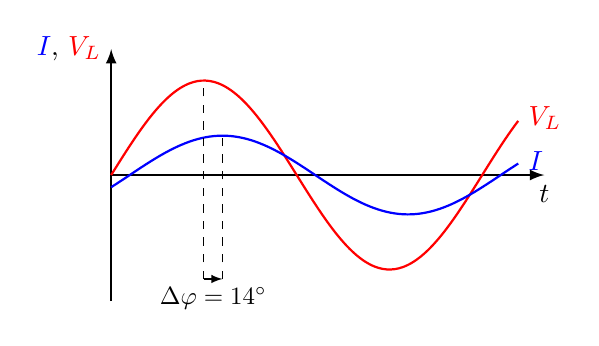
\begin{tikzpicture}
  \coordinate (O) at (0,0);
  \coordinate (X) at (\xmax,0);
  \coordinate (Y) at (0,\ymax);
  
  % AXIS
  \draw[->,thick]
    (0,-\ymax) -- (Y) node[left] {{\color{blue}$I$}, {\color{red}$V_L$}};
  \draw[->,thick]
    (O) -- (X) node[below] {$t$};
  
  % PLOT
  \draw[red, thick, samples=100,smooth,variable=\x,domain=0:0.94*\xmax]
    plot(\x,{\A*sin(\om*\x)}) node[above=1,right] {$V_L$};
  \draw[blue, thick, samples=100,smooth,variable=\x,domain=0:0.94*\xmax]
    plot(\x,{\I*sin(\om*\x-18)}) node[above=1,right] {$I$};
  
  % PHASE DIFFERENCE
  \draw[dashed] ({90/\om},-1.1*\A) -- ({90/\om},\A);
  \draw[dashed] ({108/\om},-1.1*\A) -- ({108/\om},\I);
  \draw[->] ({90/\om},-1.1*\A) --++ ({18/\om},0) node[midway,below,scale=0.9] {$\Delta\varphi = \SI{14}{\degree}$};
  
\end{tikzpicture}

\end{document}